\documentclass[../slides.tex]{subfiles}
\begin{document}
\section{When is commitment good/bad?}
\begin{frame}{General symmetric $2\times2$ game}
\centering
\renewcommand{\arraystretch}{1.25}
\begin{tabular}{ccc}
  % original game
  \begin{tabular}{c|cc}
      & $A_1$ & $A_2$\\\hline
    $A_1$ & $(A,A)$ & $(B,C)$\\
    $A_2$ & $(C,B)$ & $(D,D)$
  \end{tabular}
  &
  \hspace{1.2em}
  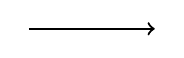
\begin{tikzpicture}[baseline=(current bounding box.center)]
    \draw[thick,->] (0,0)--(1.6,0);
  \end{tikzpicture}
  \hspace{1.2em}
  % standardised game
  \begin{tabular}{c|cc}
        & $A_1$ & $A_2$ \\[0.2em]
        \hline
        $A_1$ & $(0,0)$ & $(\bparam,\cparam)$ \\[0.2em]
        $A_2$ & $(\cparam,\bparam)$ & $(1,1)$ \\[0.2em]
    \end{tabular}
\end{tabular}

\medskip
\begin{itemize}
  \item Positive affine transform: subtract $A$, divide by $D-A$.
  \item Parameters $b=\frac{B-A}{D-A}$ and $c=\frac{C-A}{D-A}$ fully
        locate the game in \((b,c)\)-space.
\end{itemize}
\end{frame}
\begin{frame}{$(b,c)$‐space and classic $2\times2$ games}
\centering
\resizebox{0.5\linewidth}{!}{%
\begin{tikzpicture}
  \begin{axis}[
    width=10cm,height=10cm,
    axis x line=middle, axis y line=middle,
    axis line style={ultra thick},
    xlabel={$\cparam$}, ylabel={$\bparam$},
    xmin=-1,xmax=2, ymin=-1,ymax=3,
    xtick={0,1}, ytick={0,1},
    tick label style={font=\small}, label style={font=\small},
    clip=false]
    % split lines
    \addplot[black!70, thin] coordinates {(-1,1) (2,1)};
    \addplot[black!70, thin] coordinates {(1,1) (1,3)};
    % shaded strict-domination regions
    \fill[pattern=north east lines, pattern color=gray!55]
      (axis cs:-1,1)--(axis cs:0,1)--(axis cs:0,3)--(axis cs:-1,3)--cycle;
    \fill[pattern=north east lines, pattern color=gray!55]
      (axis cs:2,1)--(axis cs:0,1)--(axis cs:0,-1)--(axis cs:2,-1)--cycle;
    % labels
    \node at (axis cs:-0.5,0.5)  {\large\textbf{Stag Hunt}};
    \node at (axis cs:-0.5,-0.5){\large\textbf{Coordination}};
    \node[align=center] at (axis cs:1.5,2) {\large\textbf{Battle}\\\large\textbf{of Sexes}};
    \node[align=center] at (axis cs:0.5,2) {\large\textbf{Chicken}};
  \end{axis}
\end{tikzpicture}}
\vspace{1ex}

\scriptsize\itshape
Shaded regions denote games with dominated strategies
\end{frame}
\begin{frame}{Proposition 1}
\begin{block}{Proposition}
Consider a symmetric \(2\times2\) game and its commitment variant.  
In the unique mixed subgame perfect equilibrium of the commitment game, the expected payoff for both players relative to the mixed equilibrium of the base game is:
\begin{enumerate}
    \item weakly lower in the Game of Chicken (strictly for \(c<1)\);
    \item higher in the Battle of Sexes.
\end{enumerate}
\end{block}
\end{frame}
\begin{frame}{Corollary 1}
\begin{block}{Corollary}
The following results hold for the Coordination Game and the Stag Hunt.
\begin{enumerate}
    \item There is a mixed subgame perfect equilibrium in the Coordination Game. However, players committing to \((A_1,A_1)\) is another symmetric subgame perfect equilibrium that Pareto-dominates the mixed equilibrium.
    \item The Stag Hunt game does not have a mixed equilibrium.
\end{enumerate}
\end{block}
\end{frame}
\end{document}